\chapter[Related Work]{Related Work}
\par Presentation skills give us the power to change the world. Great presenters instill trust, engage our minds and hearts, deliver ideas and information, and inspire and captivate us.

\par In this paper, we propose a presentation training system that allow trainees to imitate past famous speech to improve their nonverbal behaviors. Many papers discussed some approaches toward the automatic recognition of nonverbal from trainees. However these approaches all defined some exact rules in advance to give a score of the presentation, but few have focused on imitating past famous speech to refine their nonverbal behaviors. Some researches analyze some visual and vocal channels of trainees, thus can provide information about their presentations. For example, the system in Pfister was originated from a vocal emotion detection module \cite{pfister2011real}. It was similar to the approach of Silverstein \cite{Silverstein2006}, which was built solely on vocal cues, by analyzing the voice such as pitch or tempo. The Hincks's system measured the changes in vocal pitch, and then give visual feedbacks to promote pitch variation by relying on the importance of pitch variance in oral presentations \cite{hincks2009promoting}.
\par On the other hand, some include nonverbal behaviors in the analysis. Gao introduced the method based only on visual information \cite{Gao}. In contrast, Kurihara added face position and orientation as the approximation of eye contact, together with pitch, speaking rate, utterance and filled pauses \cite{Kurihara2007}. Hoque proposed a automated conversation coach to help trainees improve their interview skills by recognize their motion and facial expression \cite{Kurihara2007}.
\par We will introduce the detail about Kurihara's research \cite{Kurihara2007} in section 2.2.1 and Nguyen's research \cite{nguyen2015intelligent} in section 2.2.2. 

\subsection{Presentation Sensei}
\par In Kurihara's paper they present a presentation training system that observes a presentation rehearsal and provides recommendations for improving the delivery of the presentation, such as to speak more slowly and to keep eye contact with the audience (Figure \ref{fig:sensei}). Kurihara intentionally focus on the basic behavior patterns because high-level semantics is very difficult to analyze by computers in contrast to basic behavior patterns. Kurihara's goal is to help people improve their base-line presentation skills by reducing inappropriate behavior such as using many fillers (e.g. “er”) or continuously looking down at the script.

\begin{figure}[htbp]
  \centering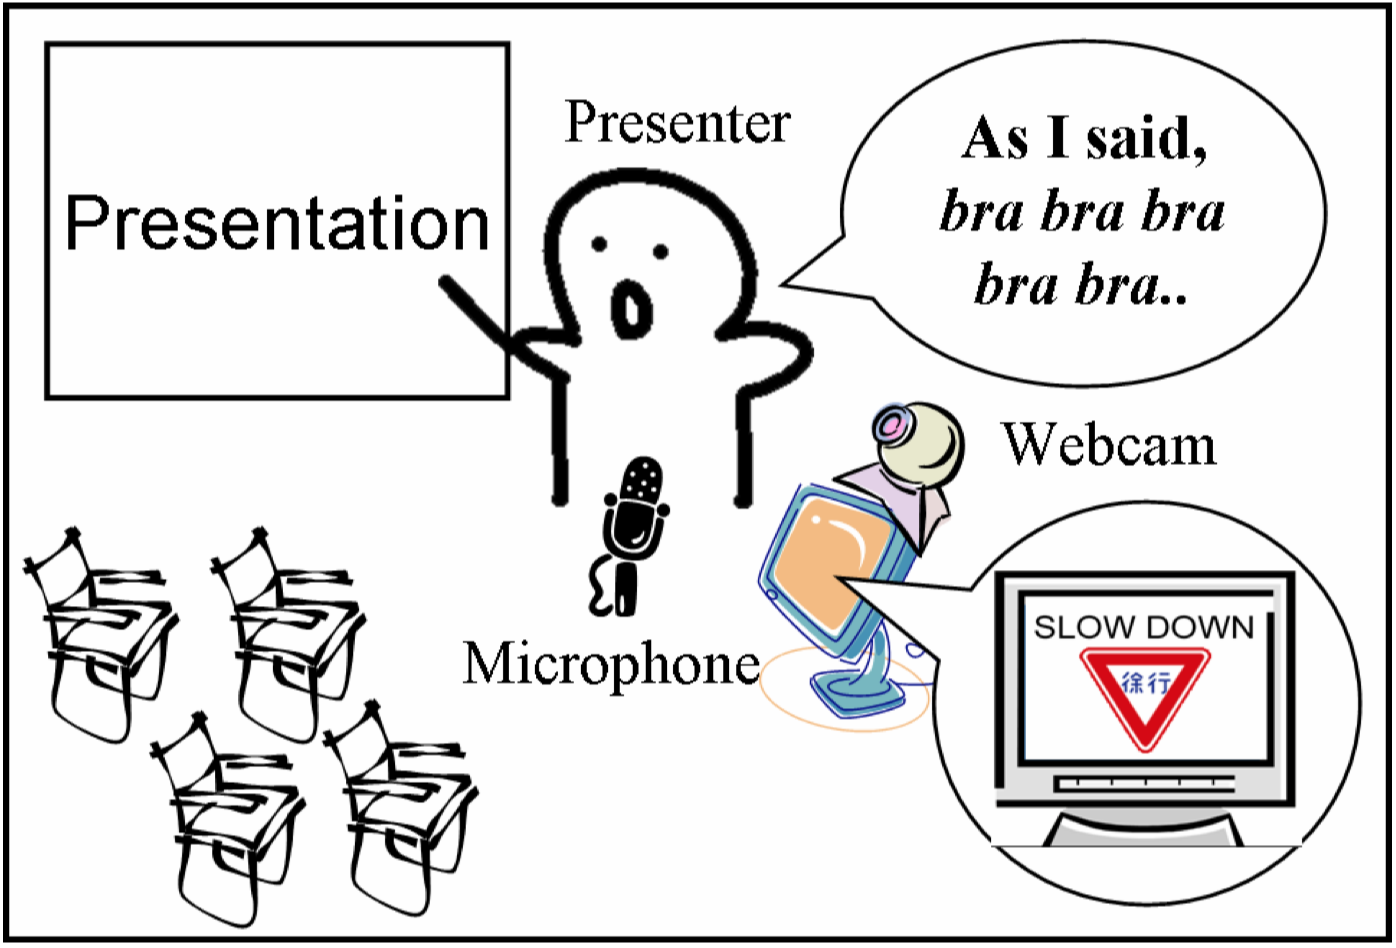
\includegraphics[width=0.8\textwidth]{./img/sensei.png}
  \caption[Presentation sensei system]{Presentation sensei system \cite{Kurihara2007}}
  \label{fig:sensei}
\end{figure}

\par In this work, Kurihara focus on the following five aspects of presentation delivery.
\begin{itemize}
  \item The speaking rate should not be too fast.
  \item The speech should not be monotonous.
  \item The speech should not contain too many fillers.
  \item The speaker should look at the audience and avoid continuously looking down at a script or a screen.
  \item The speaker should finish the presentation within a certain time limit.
\end{itemize}

\par Kurihara selected these because they are emphasized in existing literature and they can be detected to some extent using current speech processing and image processing technologies. The Presentation Sensei system visualizes the analysis result in real time communicating with a presentation tool. It can give the presenter both instant “online” feedback and post “offline” feedback for improvements. The online feedback function shows the analysis result in real-time. When the system detects some inappropriate behavior, it alerts the presenter by showing a visual signal (Figure \ref{fig:onlinefeedback}). The offline feedback function shows the visual summaries of the indices for the presenter’s self-examinations (Figure \ref{fig:offlinefeedback}).

\begin{figure}[htbp]
  \centering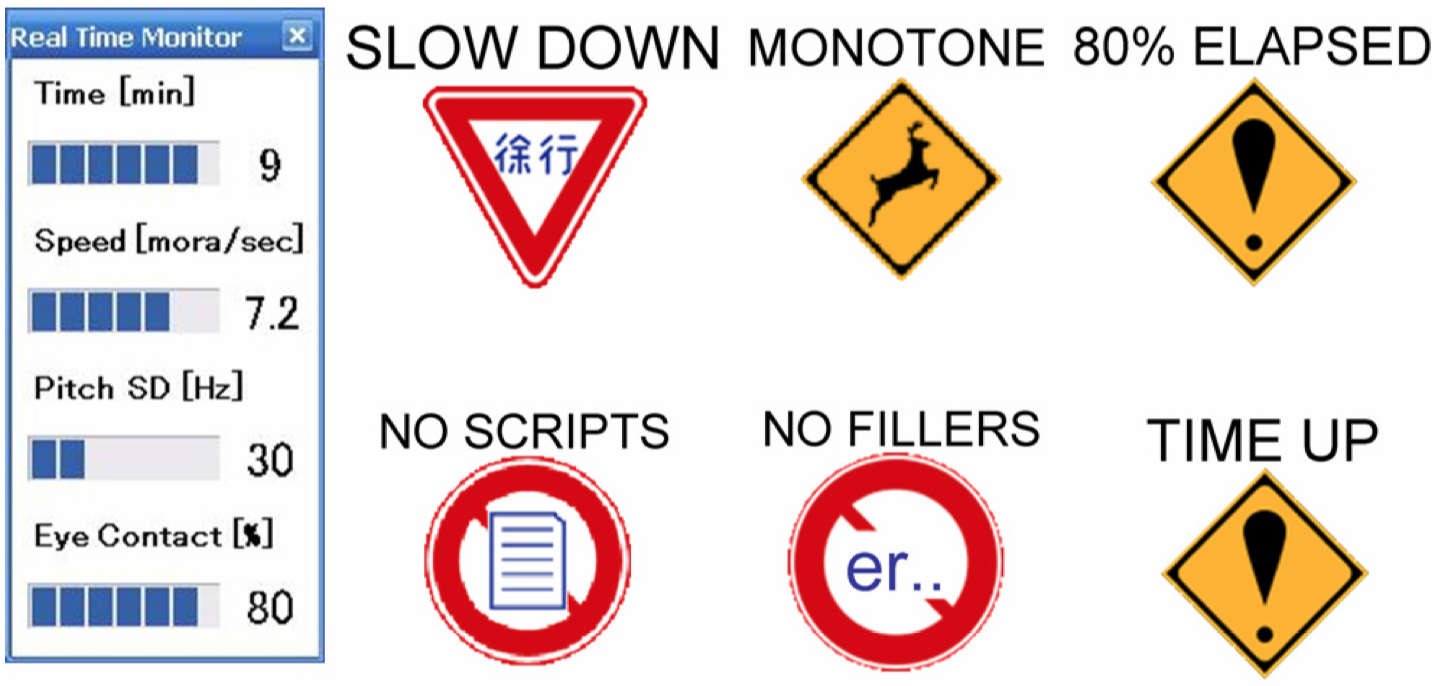
\includegraphics[width=0.5\textwidth]{./img/onlinefeedback.png}
  \caption[Online feedback of presentation sensei]{Online feedback. (Left) Real time monitor. (Trafic signals) Visual Alerts.\cite{Kurihara2007}}\label{fig:onlinefeedback}
\end{figure}

\begin{figure}[htbp]
  \centering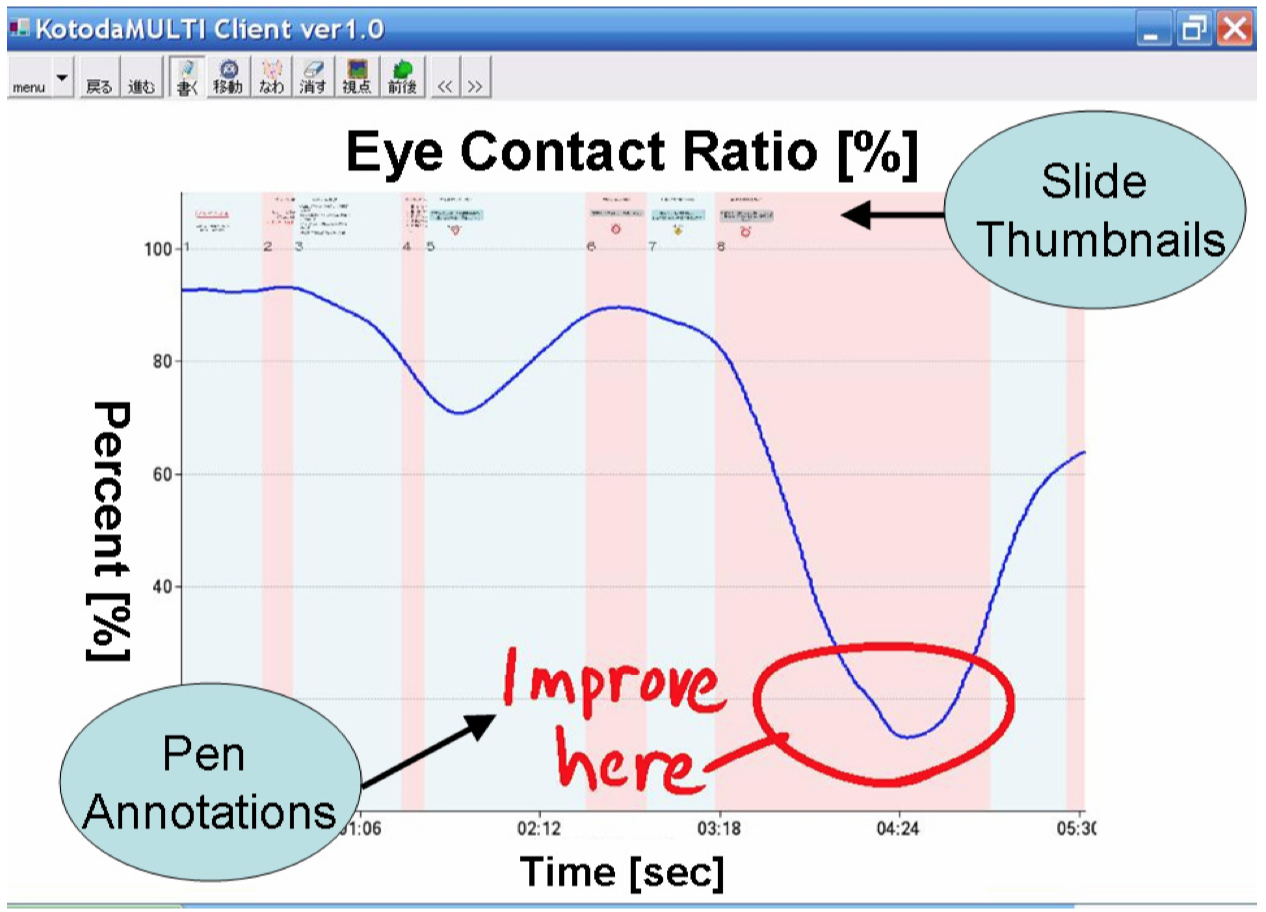
\includegraphics[width=0.5\textwidth]{./img/offlinefeedback.png}
  \caption[Offline feedback of presentation sensei]{Offline feedback. An example of the generated charts\cite{Kurihara2007}.}\label{fig:offlinefeedback}
\end{figure}

\par It is often difficult to make speech processing and image processing work robustly in adverse environments. One advantage of Kurihara's target application domain, personal presentation rehearsal, is that we can relatively freely configure the environment. It is realistic to rehearse in a silent room with no visual obstacles, where these technologies perform the best. This feature makes the Presentation Sensei system a highly practical application even with imperfect recognition technologies \cite{Kurihara2007}.
\par Kurihara's system is unique in that, while general multimodal systems help the user to control computers, it tries to help computers guide humans. This way of using a computer is relatively new. Heer et al. \cite{Heer} investigated the design guidelines for this sort of systems and also introduced an experimental media capture system that acts as a film director. 
\subsection*{System Configuration}
\par The Presentation Sensei system consists of several modules connected by a network (Figure \ref{fig:senseisystem}). The audio analysis module continuously analyses the input signal from a microphone and provides the integration module with the results of the utterance duration detection, pitch (F0) detection, and filled pause detection. The speech recognition module also continuously provides the integration module with the mora-based speech recognition results. The image processing module continuously analyzes the input from a webcam and provides the integration module with the result of the face position/orientation detection. The integration module integrates all the provided information and gives feedback to the presenter using various monitors. These modules can be distributed over a local network for the load sharing purpose and they communicate with each other via RVCP protocol \cite{Goto2001}. The system can also be connected to a third party presentation tool to achieve synchronization. Kurihara currently connect their system to an in-house presentation program to receive timing information and thumbnail images of slides.

\munepsfig[width=0.8\textwidth]{senseisystem}[System configuration of presentation sensei]{System configuration of presentation sensei \cite{Kurihara2007}}

\subsection{Intelligent Presentation Skills Trainer}
\par Nguyen's research developed a tutoring system for public speaking, which assesses presentations based solely on the visual behaviors of presenters. Firstly, an empirical study was performed in order to investigate on the nonverbal cues that impact a presentation, serving as the ground truth. Next, a Microsoft Kinect was implemented for capturing skeletal representations of the presenters' body as input data for the analysis. The recognition process can detect if the behaviors appeared in real-time. Multi-class support vector machine was used to classify the quality of presentations into a four-degree scale with the recognition rate of 73.9\% on a training/test database that includes 76 presentations. For the feedback, the system allows presenters to review their presentation, together with the analysis results. They also developed a simulated conference room as the real-time feedback mechanism.
\subsection*{Automatic Feedback System}
\par In order to support presenters with an effective solution that can help them self-practice even at home, Nguyen aimed to implement the system with the following functions: (1)Automatic analyzes presenters performance; (2)Provides immediate feedback during the presentation; (3)Provides overall analysis about the whole presentation; (4)Lets users review their performance together with the analyzed results, thus allows them to keep track of their practicing progress. In order to achieve these purposes, they set up a Microsoft Kinect to extract body's skeletal representation as input for the analysis task. In parallel, a regular camera or webcam is positioned to simulate the audiences point of view. The automatic analysis, as well as recording is processed in real-time using a regular PC. The result is visualized on the PC or an external screen/projector (Figure \ref{fig:nguyensystem}). Users also have the chance to review their presentations, together with in-depth analysis about nonverbal cues in the end.
\munepsfig[width=0.5\textwidth]{nguyensystem}[Setup of the Nguyen's system]{Setup of the Nguyen's system \cite{nguyen2015intelligent}}

\subsection*{The Two Methods of Giving Feedbacks}
\par Nguyen's system provides two ways of delivering feedbacks to the audience \cite{nguyen2015intelligent}. The first one shows users their recorded presentation, the appearances of each behaviors and results on the four nonverbal aspects, plus the overall result. In parallel, with purpose to give presenters the helpful feedbacks, also aim to provide them the experience as presenting for the real audience, Nguyen developed a virtual conference room as one method to deliver feedbacks. The environment was built using the Unity3D engine, simulates the classroom that we collected data for observation. Avatars are able to perform several animations that may bring either positive or negative feeling for presenters. These animation clips are sorted based on the increase of negative feeling: (1) Nodding; (2) Sitting still; (3) Sleeping; (4) Yawning.


\munepsfig[width=0.6\textwidth]{feedback_n}[The simulated conference room]{The simulated conference room \cite{nguyen2015intelligent}}
